\documentclass[14pt]{extbook}
\usepackage{multicol, enumerate, enumitem, hyperref, color, soul, setspace, parskip, fancyhdr} %General Packages
\usepackage{amssymb, amsthm, amsmath, bbm, latexsym, units, mathtools} %Math Packages
\everymath{\displaystyle} %All math in Display Style
% Packages with additional options
\usepackage[headsep=0.5cm,headheight=12pt, left=1 in,right= 1 in,top= 1 in,bottom= 1 in]{geometry}
\usepackage[usenames,dvipsnames]{xcolor}
\usepackage{dashrule}  % Package to use the command below to create lines between items
\newcommand{\litem}[1]{\item#1\hspace*{-1cm}\rule{\textwidth}{0.4pt}}
\pagestyle{fancy}
\lhead{Makeup Progress Quiz -1}
\chead{}
\rhead{Version A}
\lfoot{7547-2949}
\cfoot{}
\rfoot{Fall 2020}
\begin{document}

\begin{enumerate}
\litem{
To estimate the one-sided limit of the function below as $x$ approaches 7 from the right, which of the following sets of numbers should you use?\[ \frac{\frac{7}{x} - 1}{x - 7} \]\begin{enumerate}[label=\Alph*.]
\item \( \{ 7.0000, 7.1000, 7.0100, 7.0010 \} \)
\item \( \{ 6.9000, 6.9900, 6.9990, 6.9999 \} \)
\item \( \{ 6.9000, 6.9900, 7.0100, 7.1000 \} \)
\item \( \{ 7.0000, 6.9000, 6.9900, 6.9990 \} \)
\item \( \{ 7.1000, 7.0100, 7.0010, 7.0001 \} \)

\end{enumerate} }
\litem{
Based on the information below, which of the following statements is always true?\[ As $x$ approaches $\infty$, $f(x)$ approaches $12.948$. \]\begin{enumerate}[label=\Alph*.]
\item \( f(x) \text{ is close to or exactly } 12.948 \text{ when } x \text{ is large enough}. \)
\item \( f(x) \text{ is undefined when } f(x) \text{ is large enough}. \)
\item \( f(x) \text{ is close to or exactly } \infty \text{ when } x \text{ is large enough}. \)
\item \( f(x) \text{ is undefined when } x \text{ is large enough}. \)
\item \( \text{None of the above are always true.} \)

\end{enumerate} }
\litem{
Evaluate the limit below, if possible.\[ \lim_{x \rightarrow 3} \frac{\sqrt{9x - 11} - 4}{8x - 24} \]\begin{enumerate}[label=\Alph*.]
\item \( 0.016 \)
\item \( 0.125 \)
\item \( \infty \)
\item \( 0.141 \)
\item \( \text{None of the above} \)

\end{enumerate} }
\litem{
Evaluate the one-sided limit of the function $f(x)$ below, if possible.\[ \lim_{x \rightarrow -8^+} \frac{-2}{(x-8)^7}+1 \]\begin{enumerate}[label=\Alph*.]
\item \( f(-8) \)
\item \( \infty \)
\item \( -\infty \)
\item \( \text{The limit does not exist} \)
\item \( \text{None of the above} \)

\end{enumerate} }
\litem{
To estimate the one-sided limit of the function below as $x$ approaches 4 from the right, which of the following sets of numbers should you use?\[ \frac{\frac{4}{x} - 1}{x - 4} \]\begin{enumerate}[label=\Alph*.]
\item \( \{ 4.0000, 3.9000, 3.9900, 3.9990 \} \)
\item \( \{ 3.9000, 3.9900, 4.0100, 4.1000 \} \)
\item \( \{ 4.1000, 4.0100, 4.0010, 4.0001 \} \)
\item \( \{ 3.9000, 3.9900, 3.9990, 3.9999 \} \)
\item \( \{ 4.0000, 4.1000, 4.0100, 4.0010 \} \)

\end{enumerate} }
\litem{
Evaluate the one-sided limit of the function $f(x)$ below, if possible.\[ \lim_{x \rightarrow 5^+} \frac{-5}{(x-5)^7}+6 \]\begin{enumerate}[label=\Alph*.]
\item \( f(5) \)
\item \( \infty \)
\item \( -\infty \)
\item \( \text{The limit does not exist} \)
\item \( \text{None of the above} \)

\end{enumerate} }
\litem{
For the graph below, find the value(s) $a$ that makes the statement true: $ \displaystyle \lim_{x \rightarrow a} f(x) = -\infty$.
\begin{center}
    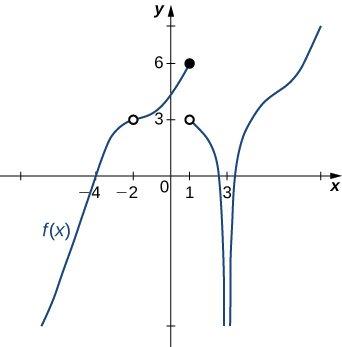
\includegraphics[width=0.5\textwidth]{../Figures/evaluateLimitGraphicallyCopyA.png}
\end{center}
\begin{enumerate}[label=\Alph*.]
\item \( -2 \)
\item \( 3 \)
\item \( -\infty \)
\item \( \text{Multiple } a \text{ make the statement true}. \)
\item \( \text{No } a \text{ make the statement true}. \)

\end{enumerate} }
\litem{
For the graph below, find the value(s) $a$ that makes the statement true: $ \displaystyle \lim_{x \rightarrow a} f(x) = 0$.
\begin{center}
    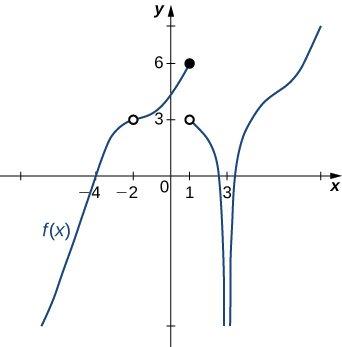
\includegraphics[width=0.5\textwidth]{../Figures/evaluateLimitGraphicallyA.png}
\end{center}
\begin{enumerate}[label=\Alph*.]
\item \( 0 \)
\item \( -4 \)
\item \( 3 \)
\item \( \text{Multiple } a \text{ make the statement true}. \)
\item \( \text{No } a \text{ make the statement true}. \)

\end{enumerate} }
\litem{
Evaluate the limit below, if possible.\[ \lim_{x \rightarrow 9} \frac{\sqrt{6x - 18} - 6}{7x - 63} \]\begin{enumerate}[label=\Alph*.]
\item \( 0.083 \)
\item \( 0.012 \)
\item \( \infty \)
\item \( 0.350 \)
\item \( \text{None of the above} \)

\end{enumerate} }
\litem{
Based on the information below, which of the following statements is always true?\[ $f(x)$ approaches $4.772$ as $x$ approaches $9$. \]\begin{enumerate}[label=\Alph*.]
\item \( f(9) = 4 \)
\item \( f(4) \text{ is close to or exactly } 9 \)
\item \( f(4) = 9 \)
\item \( f(9) \text{ is close to or exactly } 4 \)
\item \( \text{None of the above are always true.} \)

\end{enumerate} }
\end{enumerate}

\end{document}